\documentclass[english, twocolumn, 10pt, aps, superscriptaddress, floatfix, prb, citeautoscript]{revtex4-1}
\pdfoutput=1
\usepackage[utf8]{inputenc}
\usepackage[T1]{fontenc}
\usepackage{verbatim}
\usepackage{units}
\usepackage{mathtools}
\usepackage{amsmath}
\usepackage{amssymb}
\usepackage{graphicx}
\usepackage{wasysym}
\usepackage{layouts}
\usepackage{siunitx}
\usepackage{bm}
\usepackage{xcolor}
\usepackage[colorlinks, citecolor={blue!50!black}, urlcolor={blue!50!black}, linkcolor={red!50!black}]{hyperref}
\usepackage{bookmark}
\usepackage{tabularx}
\usepackage{microtype}
\usepackage{babel}
\hypersetup{pdfauthor={Quantum Tinkerer},pdftitle={Increasing the topological gap by an order of magnitude through the geomerty for Majorana SNS junctions.}}

\setcounter{secnumdepth}{4}
\setcounter{tocdepth}{4}

\DeclareMathOperator{\e}{e}
\DeclareMathOperator{\de}{d\!}
\DeclareMathOperator{\Tr}{Tr}
\DeclareMathOperator{\diag}{diag}
\DeclareMathOperator{\Res}{Res}
\DeclareMathOperator{\sgn}{sgn}
\DeclareMathOperator{\Pf}{Pf}
\DeclareMathOperator{\Det}{Det}
\DeclareMathOperator{\rank}{rank}
\DeclareMathOperator{\im}{Im}
\DeclareMathOperator{\re}{Re}
\newcommand{\kx}{k_x}
\newcommand{\ky}{k_y}
\newcommand{\meff}{m_\text{eff}}

\renewcommand{\comment}[2]{#2}
% Uncomment the following line for paragraph descriptions to appear in the file.
\renewcommand{\comment}{\paragraph}

\DeclarePairedDelimiter\abs{\lvert}{\rvert}
\DeclarePairedDelimiter\norm{\lVert}{\rVert}

\makeatletter
\let\oldabs\abs
\def\abs{\@ifstar{\oldabs}{\oldabs*}}
\let\oldnorm\norm
\def\norm{\@ifstar{\oldnorm}{\oldnorm*}}
\makeatother

\newcommand{\ev}[1]{\langle#1\rangle}
\newcommand{\bra}[1]{\langle#1|}
\newcommand{\ket}[1]{|#1\rangle}
\newcommand{\bracket}[2]{\langle#1|#2\rangle}

\newcolumntype{L}[1]{>{\raggedright\arraybackslash}p{#1}}
\newcolumntype{C}[1]{>{\centering\arraybackslash}p{#1}}
\newcolumntype{R}[1]{>{\raggedleft\arraybackslash}p{#1}}


\begin{document}


\title{Increasing the topological gap by an order of magnitude through the geometry for Majorana SNS junctions.}

\author{Quantum Tinkerer}
\affiliation{Kavli Institute of Nanoscience, Delft University of Technology, P.O. Box 4056, 2600 GA Delft, The Netherlands}
\email[Electronic address: ]{quantumtinkerer@tudelft.nl}

\date{\today}
\begin{abstract}
We solve the problem of soft gap in high density SNS Majorana junctions \cite{pientka2017topological}.
Trajectories that do not encounter the superconductor for a long time weaken proximity effect in Josephson junctions.
A small induced gap becomes then an important obstacle in creating Majorana states.
We show that a zigzag-shaped geometry eliminates these trajectories, at the same time allowing robust creation of Majorana states with a gap increased by more than an order of magnitude.
\end{abstract}

\maketitle

%%██████████████████████████████████████████████████████████████████████████
%%██ Introduction
%%██████████████████████████████████████████████████████████████████████████
\section{Introduction}
Majorana bound states (MBSs) are a promising candidate to form the basis of a stable platform for topological quantum computing.

\comment{Majoranas are mostly made in hybrid NS structures.}
The current experimental effort focuses on creating pairs of MBSs in hybrid normal-superconductor (NS) structures, where a long strip (or wire) of a semiconductor is interfaced with a \cite{lutchyn_majorana_2010,oreg_helical_2010} superconductor.
Within the right parameter regime ($E_z^2>\mu^2+\Delta^2$ for a simple wire), the semiconductor becomes topological while MBSs appear at the ends of the segment.
Recently, a system with a slight modification has been proposed\cite{pientka2017topological}, where instead of having one superconductor, there are two superconductors, creating a superconductors-normal-superconductor (SNS) junction.
The additional superconductor adds an extra knob to adjust, the superconducting phase difference $\phi$, and this should make it easier to tune the system into the topological phase.
In practice, multiple problems arise making even the observation, let alone the manipulation of Majoranas difficult.

\comment{The gap is small because of long trajectories.}
One of the biggest challenges in creating stable Majoranas is the appearance of a soft gap; where the gap in the density of states significantly reduces for states with the momentum directed along the length of the strip.
From a semiclassical perspective, these momenta correspond to long paths through the semiconductor without interruption by the superconductor.
Additionally, these long trajectories have long flight times $\tau_f$ and equivalenly small Thouless energies $E_{\textrm{Th}}=\hbar / \tau_f$, resulting in a small gap.

\comment{Currently proposed workarounds are low density or disorder, but both have drawbacks.}
Currently, proposed workarounds are to work at low density \cite{nijholt2015orbital} or to have disorder~\cite{haim_double-edge_2018}, but both have drawbacks.

\comment{We show that zigzag geometry solves this problem by eliminating the long trajectories.}
In this paper, we show that introducing a zigzag or snake-like geometry for the semiconductor eliminates these long trajectories and prevents the appearance of a soft gap while also increasing the topological gap by an order of magnitude.


%%██████████████████████████████████████████████████████████████████████████
%%██ Physical picture
%%██████████████████████████████████████████████████████████████████████████
\section{Physical picture}

\begin{figure}[!htb]
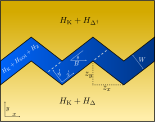
\includegraphics[width=0.95\columnwidth]{figures/zigzag.pdf}
\caption{Setups. Figure of a straight and zigzag system, including trajectories.
\label{fig:setup}}
\end{figure}

\comment{We consider a two-dimensional system with zigzag.}
We consider a Josephson junction (JJ)(Fig.~\ref{fig:setup}) consisting of a two-dimensional strip of semiconductor, with superconductors on both sides.
We modulate the shape of the normal region, which can be either zigzag as depicted, or a more smooth sinusoidal-like shape.
Similar to the conventional straight system \cite{pientka2017topological}, a magnetic field $B_x$ perpendicular to the junction is applied.
We model the system with a BdG Hamiltonian Eq.~\eqref{eq:hamiltonian}; the normal part has a linear Rashba spin-orbit coupling term characterized by $\alpha$ and a Zeeman field with $E_z=\frac{1}{2} \mu_B g B_x$.
The superconductor has a superconducting coupling term $\Delta$ with a superconducting phase $\exp{\pm i \phi/2}$.
Both parts have a kinetic term and chemical potential $\mu$.
For the zigzag geometry, we first consider a sawtooth-like pattern where $z_x$ is periodicity, $z_y$ the amplitude and $W$ the width of the junction.
Later in this manuscript, we show that the exact details of the shape are unimportant and consider different zigzag geometries also parametrized by $z_x, \; z_y, \; W$.

\begin{small}
\begin{align}
    H = \left(\frac{\hbar^2\left(\kx^2 + \ky^2\right)}{2\meff} - \mu\right)\tau_z+
        E_\text{z} \sigma_x+
        \alpha \left( \ky \sigma_x - \kx \sigma_y \right) \tau_z +
        \Delta \tau_y
\end{align}
\label{eq:hamiltonian}
\end{small}

Unless noted differently, the Hamiltonian parameters are $\alpha=\SI{20}{\meV \nm}$, $g=26$, $\meff=\SI{0.02}{\electronmass}$, $\mu=\SI{10}{\meV}$, $B=\SI{1}{T}$, $\phi=\pi$, and $\Delta=\SI{1}{\meV}$; and the geometry parameters are $W=\SI{200}{\nm}$, the period of the zigzag $z_x=\SI{1300}{\nm}$, the discretization contant $a=\SI{10}{\nm}$, and the lengths of the superconductors $L_\textrm{SC}=\SI{200}{\nm}$.

%%██████████████████████████████████████████████████████████████████████████
%%██ Calculating the bandstuctures
%%██████████████████████████████████████████████████████████████████████████
\section{Calculating the bandstuctures.}\label{sec:bandstuctures}

\comment{We discretize the Hamiltonian and simulate it with Kwant.}
We discretize our continuum Hamiltonian \eqref{eq:hamiltonian} on a square grid and implement a tight-binding model using Kwant~\cite{groth_kwant:_2014}.
The resulting Hamiltonians are large because instead of having a single slice of sites that is translationally invariant in the $x$-direction, we create a long supercell to make the structure periodic.
To speed up these expensive simulations we employ an adaptive sampling strategy, using the Python package Adaptive. % TODO: add a citation

\begin{figure}[!htb]
\includegraphics[width=0.95\columnwidth]{figures/bandstructures}
\caption{Figure of the bandstuctures corresponding to the system in Fig.~\ref{fig:setup}.
Blue lines correspond to $\phi=0$, $B=0$ and red lines to $\phi=\pi$, $B = \SI{1}{T}$.
The three subplots are for different amplitudes of the zigzag, with (a) $z_y=0$, (b) $z_y=\frac{W}{4}$, and (c) $z_y=\frac{W}{2}$, where $W=\SI{200}{\nm}$ is the junction width.
We observe that once there are no more straight trajectories inside the junction (when $z_y=\frac{W}{2}$) the spectrum becomes most insensitive to the momentum $k_x$.
The parameters values are as noted below Eq.~\eqref{eq:hamiltonian}.\label{fig:bandstuctures}}
\end{figure}

\comment{We calculate the bandstructure for varying amount of zigzag.}
In figure~\ref{fig:bandstuctures}, the bandstructure for zigzag systems with varying amplitude is displayed.
Because the discretized zigzag system is modeled using a supercell, we can only plot a folded bandstructure.
For comparison's sake, we take the same cell size for the ribbon structure such that the bandstructure folds in the same way.

\comment{The band structures show that modulation of the geometry increases the gap by an order of magnitude, as well as reduce the group velocity.}
The introduction of a zigzag has a striking effect: the bands flatten out, and more importantly, the topological gap increases by more than an order of magnitude.
On an intuitive level we can understand this because in a straight system long trajectories are possible, these have a momentum that is directed along the strip and consequently, $k_x \approx k_F$.
Further, the smallest gap in a straight system occurs around $k_F$, and because the zigzag cuts off long trajectories, the gap size increases.
Besides this, the velocity of the modes greatly reduces, which has a positive effect on the Majorana coherence length, as described later in section \ref{sec:shape_effects}.

\comment{The introduction of an NS interface at many angles increases the transparency.}
Additionally, in the presence of normal reflection, due to the presence of NS interfaces at a wide range of angles, the reflected part will eventually scatter with a near perpendicular surface.
This means that for transversal modes the transparency of the NS interface will increase.


%%██████████████████████████████████████████████████████████████████████████
%%██ Analytical estimate
%%██████████████████████████████████████████████████████████████████████████
\section{Analytical estimate of the band gap}

\comment{To compute the effect of cutoff consider a single segment of the zigzag and obtain the spectrum analytically (this allows to use translation invariance).}
We establish that the cutoff of long trajectories is the driving mechanism behind the order of magnitude gap improvement using an analytical approach.
We derive the Andreev spectrum for a single (diagonal) segment of the zigzag, and define the gap of the system as the minimum of the spectrum occurring before the cutoff corresponding to the particular geometry.
The system under consideration is thus a ribbon SNS junction with a tilted magnetic field.

\comment{The definition of the cutoff...}

\comment{We use a short junction approximation and neglect transverse SO.}
We derive the spectrum by calculating the scattering matrix for the normal region and applying the Andreev bound state condition for the short junction limit\cite{beenakker1991universal, sticlet_robustness_2017}.
For derivation of the scattering matrix, we neglect SOI in the transverse direction, which is valid for $W<l_\text{so}$.
The result is specified in Eqs.~\eqref{eq:smatrix} to~\eqref{eq:momenta_short_junction}.

\begin{align}
\label{eq:smatrix}
    S &= \left(
    \begin{array}{rr}
    r_{ll}&t_{rl}\\
    t_{lr}&r_{rr}\\
    \end{array}
    \right) =
    \left(
    \begin{array}{rr}
    \beta_+ & e^{-i q W} \beta_-\\
    e^{-i q W} \beta_- & e^{-2 i q W} \beta_+\\
    \end{array}
    \right)
    \\
    \beta_\pm &= \left(
    \begin{array}{rr}
    e^{i \nu_{\arg}}\left(\omega^\pm_1 - \omega^\pm_2\right) & (\omega^\pm _1 + \omega^\pm _2)\\
    -(\omega^\pm _1 + \omega^\pm _2) & e^{-i \nu _{\arg }} \left(\omega^\pm _2 - \omega^\pm _1\right)\\
    \end{array}
    \right)\\
    \omega^\pm_j &= \frac{1}{4} \left(\gamma _{j} \pm \delta _{j}\right)
\end{align}

\begin{align}
    \gamma_j &= \frac{q+i k_{j} \tan \left(\frac{W k_{j}}{2}\right)}{q-i k_{j} \tan \left(\frac{W k_{j}}{2}\right)} \\
    \delta_j &= \frac{q-i k_{j} \cot \left(\frac{W k_{j}}{2}\right)}{q+i k_{j} \cot \left(\frac{W k_{j}}{2}\right)}\\
    e^{i \nu_{\arg}} &= \frac{E_\text{z} e^{i \theta }-i \alpha  k_x}{\sqrt{E_\text{z}^2+\alpha  k_x \left(\alpha  k_x-2 E_\text{z} \sin (\theta )\right)}}
\end{align}

\begin{footnotesize}
\begin{align}
    q &= \left[ \frac{2 m_\ast}{\hbar ^2}\mu_s - k_x^2 \right]^\frac{1}{2}\\
    k_1 &= \left[ \frac{2 m_\ast}{\hbar^2} \left(\mu_n-\sqrt{E_z^2-2 \alpha  E_z \sin (\theta ) k_x+\alpha ^2 k_x^2}\right) - k_x^2 \right]^\frac{1}{2}\\
    k_2 &= \left[ \frac{2 m_\ast}{\hbar^2} \left(\mu_n+\sqrt{E_z^2-2 \alpha  E_z \sin (\theta ) k_x+\alpha ^2 k_x^2}\right) - k_x^2 \right]^\frac{1}{2}
\label{eq:momenta_short_junction}
\end{align}
\end{footnotesize}


In order to get the spectrum from the S-matrix [Eq.~\eqref{eq:smatrix}] we use the main result from Ref.~\onlinecite{beenakker1991universal} and start with a determinantal equation for the bound state energies in a SNS-junction:

\begin{equation}
\det\left[1+\alpha^{2}\left(E\right)r^{*}S_{e}\left(E,\bm{k}\right)rS_{e}^{*}\left(-E,-\bm{k}\right)\right]=0
\end{equation}

We rewrite this as a characteristic polynomial problem $\det\left[A-\lambda I\right]=0$, as

\begin{equation}
\det\left[r^{*}S_{e}\left(E,\bm{k}\right)rS_{e}^{*}\left(-E,-\bm{k}\right)-\frac{-1}{\alpha^{2}\left(E\right)}I\right]=0
\end{equation}

with
\begin{equation}
\lambda=-\frac{1}{\alpha^{2}\left(E\right)},\;A=r^{*}S_{e}\left(E,\bm{k}\right)rS_{e}^{*}\left(-E,-\bm{k}\right).
\end{equation}

Where $\lambda_i$ are the eigenvalues of $A$.
Inverting $\alpha\left(E\right)\equiv\exp\left(-i\arccos\left(E/\Delta\right)\right)$ yields $\frac{E}{\Delta}=\frac{\alpha^{2}+1}{2\alpha}=\frac{1}{2}\left(\alpha+\alpha^{-1}\right)=\textrm{Re}(\alpha)$, where the last equality holds because $\alpha$ is unitary.
Then, since $\alpha$ is only defined in the positive imaginary plane, the energies are $\frac{E_{i}}{\Delta}=\textrm{Re}\left(\sqrt{-1/\lambda_{i}}\right)$ where we take the root which has a positive imaginary part.
Using this result and Eq.~\eqref{eq:smatrix}, we numerically find the Andreev spectrum.

\comment{The lowest energy at $|k| < k_\textrm{cutoff}$ sets the band gap.}
We cut off the spectrum at the momentum corresponding to the proposed cutoff in the zigzag, and compare it to the numerically obtained gap for a true zigzag system.

%%██████████████████████████████████████████████████████████████████████████
%%██ Localization lengths and shape effect
%%██████████████████████████████████████████████████████████████████████████
\section{Localization lengths and shape effects}\label{sec:shape_effects}

\begin{figure}[!htb]
\includegraphics[width=0.95\columnwidth]{figures/wavefunctions}
\caption{Density of wavefunctions $\left|\psi\right|^2$ for sizes and geometries.
With (a) a straight system, (b) a saw-toothed zigzag system, (c) a system where the normal region is defined by lines parallel to a sinusoid, and (d) similar to (c) but with disordered edges.
Inside the figure, we indicate the Majorana length (or coherence length) $\lambda_\textrm{M}$ and the topological energy gap $E_\textrm{gap}$.
We observe that $\xi$ for (a) is significantly longer and $E_\textrm{gap} = E_\textrm{1} - E_M$ orders of magnitude smaller than for (b), (c), and (d), meaning that the details of the geometry do not matter for the improvements to occur.
The parameters values are as noted below Eq.~\eqref{eq:hamiltonian}.\label{fig:wavefunctions}}
\end{figure}

\comment{We calculate the wave functions and find the Majorana lengths by fitting an exponential.}
We model a finite system to compute the Majorana wave function density for different geometries; ribbon, saw-toothed zigzag, parallel curves, and variants of the latter with disordered edges.
By diagonalizing the Hamiltonian, we find the Majorana energy $E_\textrm{M}$ and the energy of the first excited state $E_1$, the lowest and second lowest energies, respectively.
Using the eigenstates, we calculate the Majorana decay length $\lambda_\textrm{M}$ by fitting an exponential to the density of the Majorana wavefunction projected on the $x$-axis.
In figure~\ref{fig:wavefunctions} the wavefunctions are displayed, superimposed upon their respective geometry.
All systems have identical Hamiltonian parameters in order to compare the effects of the changing geometry meaningfully.

\comment{In a straight system, the Majoranas are very poorly localized.}
For the ribbon system [Fig.~\ref{fig:wavefunctions}(a)], we see that the decay of the density is long compared to the system size.
The wavefunction extends to the center of the system, resulting in overlapping Majoranas and a non-zero energy of the state.
Further, the energy of the Majorana state $E_\textrm{M}$ in the straight system is badly septated from the next lowest lying eigenstate $E_1$.
Altogether, the increase in the topological gap, but also the before mentioned reduction of the group velocity, result in poorly localized Majoranas and minimal topological protection against perturbations.  % TODO: probably put the eq for coherence length here?

\comment{In a zigzag geometry Majoranas are localized within one segment of zigzag.}
We observe that for zigzag systems the Majorana properties improve.
All of the zigzag type geometries display a reduced coherence length and the delocalized nature of the wavefunctions is improved, as is visible through the density plots.
Quantitatively, the improvement in the localization of the Majoranas is also distinctly apparent: the energies of the Majorana states are three orders of magnitude lower than the energy of the second lowest-lying wavefunctions.
As mentioned in section \ref{sec:bandstuctures}, this can be attributed to the way the energy gap and velocity factor into the Majorana coherence length which scales with these parameters $\lambda_\textrm{M}=\hbar\frac{v_\textrm{F}}{\Delta_\textrm{ind}}$.
Additionally, the reduction of the Majorana decay length allows for shorter systems sizes, which is favorable because in an experimental device the coherence length of a material sets a limit for the device size.

\comment{The specific geometry is not important.}
The shape of the wavefunctions does not change significantly depending on the details of the geometry.
The sharp corners of the sawtooth versus the smooth shape of the snakelike system do not have a significant impact on the shape of the wavefunction, and neither do the disordered edges affect the relevant parameters.

%%██████████████████████████████████████████████████████████████████████████
%%██ Calculating the topological phase diagram
%%██████████████████████████████████████████████████████████████████████████
\section{Calculating the topological phase diagram.}

\begin{figure}[!htb]
\includegraphics[width=0.95\columnwidth]{figures/phasediagrams}
\caption{Phase diagrams of a straight system (a), (b) and zigzag system (c), (d), where (a), (c) are $E(\mu, B)$ and (b), (d) are $E(\phi, B)$.
Phase diagrams of a straight system (a), (b) and zigzag system (c), (d), where (a), (c) are $E(\mu, B)$ and (b), (d) are $E(\phi, B)$.
We compute the dispersion of the translationally invariant realizations of a straight and saw-toothed zigzag system and find $\min{E(k)}$ to obtain the energy gap.
% Additionally, use a generalized eigenvalue problem to find all phase boundaries at once.
The parameters values are as noted below Eq.~\eqref{eq:hamiltonian}, except with $a=\SI{5}{\nm}$ and $L_\textrm{SC}=\SI{800}{\nm}$.
The chemical potential is $\mu=\SI{10}{\meV}$ in (b) and (d) and the superconducting phase is $\phi=\pi$ in (a) and (c).
\label{fig:phasediagrams}}
\end{figure}

\comment{We calculate the topological phase diagram using the gap size.}
Due to the large size of the system, we are unable to use full spectrum methods (like the Pfaffian) to compute the topological invariant of our system.
Instead, we calculate the energy gap by finding the absolute minimum of the spectrum $E_\textrm{gap}=\min{|E(k)|}$.
By both observing the gap closings and knowing the topological phase for the non-zigzag system, we can infer the topology of the system with zigzag modulation.
In Fig.~\ref{fig:phasediagrams}, we plot the energy gap as a function of magnetic field, chemical potential, $E_\textrm{gap}(B_x, \mu)$; and the superconducting phase difference $E_\textrm{gap}(B_x, \phi)$ for both a straight system [(a) and (b)] and a zigzag system [(c) and (d)].

\comment{The introduction of the zigzag breaks a chiral symmetry, bringing the system from the BDI to the D symmetry class}
The non-zigzag system is in the symmetry class BDI \cite{pientka2017topological}.
Using the software package Qsymm\cite{varjas2018qsymm}, we find that the symmetry class of our system to be $\mathcal{D}$ because we break the chiral symmetry $\mathcal{C}$ resulting from the mirror-symmetric junction.

\comment{The phase diagram does not change much, except we see a cleaner spectrum as a result of the D class symmetry.}
Similar to what is described by Pientka et. al~\cite{pientka2017topological}, we see that the ribbon topology has a diamond-like shape as a function of phase $\phi$ and Zeeman field $E_Z$.
We also observe additional gap closings which are due to the BDI symmetry that is present.
As expected for the zigzag system, the magnitude of the gap is significantly improved, while preserving the diamond-like shape in parameter space.
Additionally, we see a cleaner and more stable topological region due to the absence of the gap closings resulting from the aforementioned chiral symmetry.

%%██████████████████████████████████████████████████████████████████████████
%%██ Discussion and Conclusions
%%██████████████████████████████████████████████████████████████████████████
\section{Discussion and Conclusions}

\comment{The zigzag geometry is a useful tool in hardening the gap and decreasing Majorana length.}
The introduction of a zigzag geometry increases the topological gap by over an order of magnitude, as well as offering a substantial reduction of the Majorana length, which enables experimentalists to create significantly shorter devices.
Additionally, the breaking of BDI symmetry into D symmetry results in a cleaner and more stable topological region.

\comment{Current fabrication techniques are compatible with the proposed geometry, and experimental verification can be near.}
Current fabrication techniques are compatible with the proposed geometry; zigzag devices have already been fabricated. % TODO: add ref to Fokko's thesis
Slight modifications to the geometry, for example, to ease measurement, should not have significant implications on the physics.

\comment{It is interesting to study what geometry creates an optimal environment for Majorana modes to exist.}
We have studied sawtooth and snake-like geometries of the semiconductor region, but perhaps a more exotic shape will be optimal.
A study optimizing the geometry's parameters for supporting Majoranas is an exciting continuation of our research.

\comment{Extensions: we omit several physical effects, disorder, electrostatics, etc.}
Finally, we exclude several physical effects, such as disorder, electrostatics, the orbital effect, the finite thickness of the sample, and electron-electron interactions, however, we expect these to be second or higher order effects which will not alter our conclusions.

%%██████████████████████████████████████████████████████████████████████████
%%██ Acknowledgments
%%██████████████████████████████████████████████████████████████████████████
\section{Acknowledgments}
We are grateful to "people" for useful discussions.
This work was supported by the Netherlands Organization for Scientific Research (NWO/OCW), as part of the Frontiers of Nanoscience program, the Foundation for Fundamental Research on Matter (FOM), and an ERC Starting Grant STATOPINS 638760.

\bibliographystyle{apsrev4-1}
\bibliography{snakemajoranas}
\end{document}
